%
% part2.tex
%

\section{Image Filtering and Enhancement}

\subsection{Finite Difference Approximations}
\begin{align}
    f(x,y) =
    \sum_{i=I_{\text{min}}}^{I_{\text{max}}}
    \sum_{j=J_{\text{min}}}^{J_{\text{max}}}
    w(i,j) \frac{I(i + x + 1, j + y) - I(i + x - 1, j + y)}{2}
    \\
    f(x,y) =
    \sum_{i=I_{\text{min}}}^{I_{\text{max}}}
    \sum_{j=J_{\text{min}}}^{J_{\text{max}}}
    w(i,j) \frac{I(i + x, j + y + 1) - I(i + x, j + y - 1)}{2}
\end{align}

\subsection{Linearly Separable Filters}
These types of filters can be carried out row-by-row, and column-by-column,
since less pixels are affecting the intermediate results, I would think this
is what allows linearly separable filters to be more robust toward noise.

This is a guess, and I didn't have time to put more thought into it than that.

\subsection{Comparison of Mean and Median Filtering}
\begin{multicols}{2}
As we can see from figure \ref{fig:2-3-a} the median filter is much better at
reducing {\it salt and pepper} noise, whilst the mean filter (at least in my
opinion does a somewhat better job at reducing gaussian noise.

The code used to generate the graph on the left, and the image figures below
can be found in the appendix section \ref{appendix:2-3}.
    \vfill{\ }\columnbreak
    
    \begin{figure}[H]
        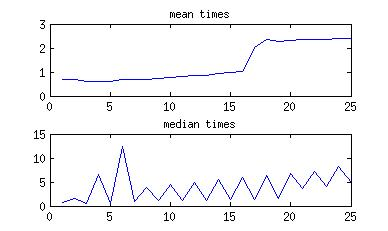
\includegraphics[scale=0.6]{figures/2-3-b.jpg}
        \caption{$x$-axis is $N$ and $y$-axis is number of sec. for 100
        computations}
        \label{fig:2-3-b}
    \end{figure}
\end{multicols}
\begin{figure}[H]
    \center
    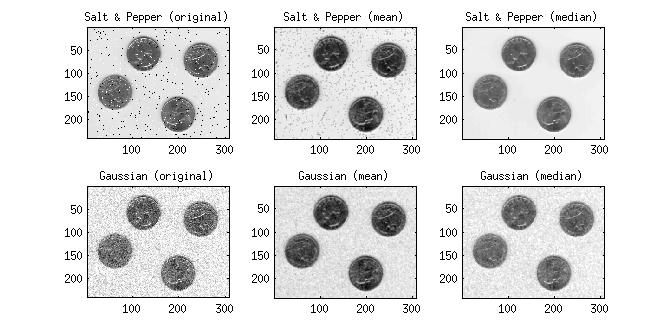
\includegraphics[scale=0.5]{figures/2-3-a.jpg}
    \caption{Showing originals (left), mean filtered (middle) and median
    filtered (right)}
    \label{fig:2-3-a}
\end{figure}

\subsection{Filter Limits}
As we increase $N$ the region affected by the filter gets so large that the
standard deviation $\sigma$ no longer has any effect. In this case, I stop
seeing any differences at approximately $N=15$.

\subsection{Standard Deviation}
Keeping $N > 3\sigma$ we let the filter continue to let the imaginary pixels
outside of the image affect the result, and as we continue to increase
$\sigma$ the image gradually moves towards a single uniform intensity across
the entire image.

